\documentclass[twoside,numberorder]{buptthesis}
%==============================================================
%==============================================================

%自己需要增加什么 package 或修改什么设置的话,都放在这里吧。
\usepackage{url}
\usepackage[colorlinks,citecolor=black,filecolor=black,linkcolor=black,urlcolor=black,bookmarksopen=true]{hyperref}
%一些全局工具的定义
\DeclareMathOperator*{\argmin}{arg\,min}
\DeclareMathOperator*{\argmax}{arg\,max}

%==============================================================
%==============================================================
\begin{document}
\pagestyle{empty}
%==============================================================
%==============================================================
\chapter*{外\quad 文\quad 译\quad 文}
\thispagestyle{empty}
\section{序贯译码技术}
序贯译码最早是由Wozencraft提出,但是被广泛应用还是因为费诺修改的算法。我们的讨论大体上集中在费诺算法上,但是,还是会与堆栈序贯译码算法做相应的对比。

一个维特比译码器延伸并更新所有潜在最好的路径度量时,而一个序贯译码器严格地限制实际要更新的路径数量。序贯译码方式的最本质思想就是仅仅延伸那些“貌似”最可能的路径。我们说“貌似”,是因为,由于搜索的限制,译码器不能完全地确定这条路径就是最好的。这种趋近方式可以看作为在码树中搜索出正确路径的试探-纠正技术。这种搜索方式,在序贯译码中总是仅仅在一个单独的路径上搜索。然而,译码器是被允许后退和改变先前决定的。每一次译码器前进都是一种“试探性”的动作。我们总是监测沿着它的最可能的路径来决定是否延伸路径。如果做出一个错误的决定,纳闷后面的路径延伸也都是错误的。译码器通过监测路径度量最终是可以察觉到这种情况的。然而,还是有延伸到错误路径的很多可能。当这种情况发生的时候,我们要消耗相当多的运算量来改正这个错误,从而进入正确的路径。译码器时常要往后搜索或者探索侧枝,直到译码最终的成功。因此,小心的选择译码参数很重要,它能使译码器快速识别错误路径并恢复到正确路径上,以便减轻运算量。序贯译码的最基本的好处就是每一次的正确路径都能够限制一定数量的计算量。同时,路径度量还是先前正确决定的指示。

在节点$i$处的分支度量定义如下:
\begin{eqnarray}
  \lambda_i=\sum_{j=1}^n\left\{\log_2 \left[\frac{P(r_i^j|t_i^j)}{P(r_i^j)}-B\right]\right\}
  \label{equ:1}
\end{eqnarray}
其中$t_i^j$是发送符号,$r_i^j$是接受符号。(假设每个分支n个符合,$R=m/n$)$k$节点的路径度量可定义为:
\begin{eqnarray}
  L_k=\sum_{i=0}^k\lambda_i
  \label{equ:2}
\end{eqnarray}
参数$B$是个偏移量,以后会详细介绍。大致上,这个变量被选中是因为,在正确路径上,度量值会增加而在错误路径上度量值会减小。尽管度量值在正确路径上由于信道噪声会短时间内下降很多,但是长时间观察,它还是增长的函数。同样的,如果信道噪声毛刺产生,在错误路径上的度量值也会短时间看起来像正确的路径,但是当噪声平息下来时,它也会开始下降。序贯译码算法能够检测出减小的度量值并能快速地找到一个增加的度量。要实现这个,它通常用动态门限T来实现。当当前的度量值小于动态门限值T的是很,它表明这条路径可能是错误的,因此将开始正确路径的搜索。
\section{费诺算法的序贯译码方式}
序贯译码器其实就是试探-纠正的一种搜索方式。费诺算法的基本译码准则是译码器不会在一条路径度量值小于当前门限的路径上前进或者后退。从当前节点延伸出来的$2^m$个分支和收到的分支比较,并根据它们最可能的概率来排序。通常,只要度量大于当前门限值,译码器就沿着最可能的节点前移。而且,如果$T+\Delta$在正确路径上可行,那么门限就增加$\Delta$。当译码器不能再前进,它试图在不减小门限的情况下后退,并且在当前门限条件下搜索其他所有没有尝试过的路径。当找不到路径能够满足当前门限时,那么门限值就下降$\Delta$,并且译码器再次向前搜索。下表就是一组关于费诺算法的准则。
\begin{table}
  \centering
  \caption{费诺准则}
  \label{tab:1}
  \begin{threeparttable}
  \begin{tabular}{ccccc}
    \hline
    \multicolumn{3}{c}{Conditions}&\multicolumn{2}{c}{Action}\\
    \hline
    Rule&Previous&Comparisons\tnote{c}&Final threshold&Move\\
    \hline
    1&F or L&$L_{k-1}<T+\Delta,L_k\ge T$&Raise(if possible)&F\\
    2&F or L&$L_{k-1}\ge T+\Delta,L_k\ge T$&No change&F\\
    3&F or L&any$L_{k-1},L_k<T$&No change&B\\
    4&B&$L_{k-1}<T,\mbox{~any~} L_k$&Lower&F\\
    5&B&$L_{k-1}\ge T,\mbox{~any~} L_k$&No change&L or B\\
    \hline
  \end{tabular}
  \begin{tablenotes}
    \footnotesize
  \item[c] By convention set $L_0=0 \mbox{~and~} L_{-1}=-\infty$
  \end{tablenotes}
\end{threeparttable}
\end{table}
表\ref{tab:1}中字母F,L和B分别代表译码器的前进,侧枝,后退动作。在前进时,译码器是前进到当前节点分出的$2^m$个节点中最可能的一个。后退则是简单地移动到当前节点先前处理的那个节点。而侧枝就是选择出了当前节点外的其他侧枝,并且是最可能的那个节点。当有少量噪声的时候,译码器会应用准则1,进而选择正确的路径。译码器能够在众多的分支中选择正确的路径前进,并且前进的路径唯一。

当判决门限比$L_k$小$\Delta$时,那么她增加,如果噪声很严重,在一个前进动作后,度量值小于门限,准则3将被应用,译码器回退,并且找到一个路径,是的度量值大于当前门限。一个回退动作后,准则4或者准则5将被应用,依据$L_{k-1}$是小于还是大于当前门限。如果$L_{k-1}\ge
T$,那么将选择最可能的侧枝节点,如果节点存在,如果不存在,那么就后退。如果$L_{k-1}<T$,不减小当前门限值而后退的动作将不成立,因此要减小$\Delta$,并且前进。译码器尝试寻找一个大于刚刚减小的门限的路径。准则2将被应用。只要$L_{k-1}\ge
T+\Delta$,那么判决门限值将不能增加,因为如果增加,译码器将会陷入一个死循环中。
\begin{figure}[htb]
  \begin{center}
    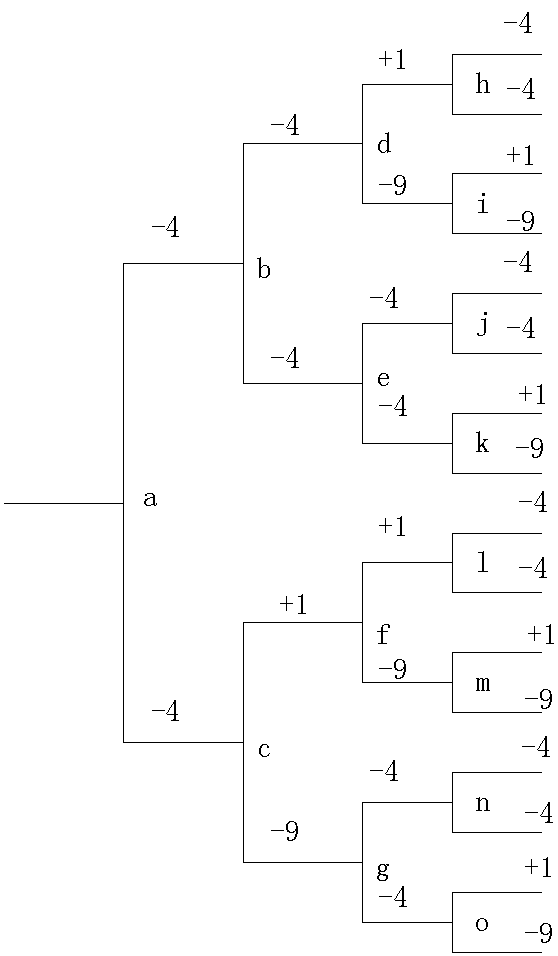
\includegraphics[width=0.4\textwidth]{tra1.pdf}
  \end{center}
  \caption{树状图实例}
  \label{fig:1}
\end{figure}
为了更好的理解费诺算法,考虑图\ref{fig:1}中码树显示$R=1/2.v=1$的码字,假设我们用的是硬判决译码算法,而且发送的码字序列是$10000\cdots$,收到的码字序列是$\mathbf{R}=01
01 00 01 00
00\cdots$,也就是说,有些单独的错误出现在第一和第四分支。表\ref{tab:2}表示的是接受码字$\mathbf{R}$依据码树产生的路径度量,其中如果码字相符度量值加$+0.5$否则度量值减$-4.5$(度量增量的选择,以后会介绍)。
\begin{table}
  \centering
   \caption{费诺算法树搜索实例}
  \label{tab:2}
  \begin{tabular}{C{3cm}C{1.5cm}C{1.5cm}C{1.5cm}C{2.5cm}C{2.5cm}}
    \hline
    Node&T&k&$L_k$&Final T&Move\\
    \hline
    b&0&1&-4&0&B\\
    a&0&0&0&-5&F\\
    b&-5&1&-4&-5&F\\
    d&-5&2&-8&-5&B\\
    b&-5&1&-4&-5&L\\
    c&-5&1&-4&-5&F\\
    f&-5&2&-3&-5&F\\
    l&-5&3&-2&-5&F\\
    o&-5&4&-6&-5&B\\
    l&-5&3&-2&-5&B\\
    f&-5&2&-3&-5&B\\
    c&-5&1&-4&-5&B\\
    a&-5&0&0&-10&F\\
    \hline
  \end{tabular}
 
\end{table}
表\ref{tab:2}中显示了费诺算法的步骤。当译码器在一个节点遇到两个度量值相同的两个分支时候,(就像第一步),那么通常都是先尝试上面的一个分支。因此,算法总是先在上半部分书寻找最好路径。第一步前进的结果导致门限失败,因此要强制后退,并且降低门限值。然而,当沿着相同方向前进到节点$d$的时候,另一次门限失败发生。这将强制后退并进入下半部分码树尝试寻找一个更好的路径。沿着这条路径前进,直到节点$p$,另外一个信道错误导致门限失败。译码器必须重新回退,直到到达节点$a$,并且降低门限值到$-10$。现在,只剩一条路径总是大于这个门限值。再搜索上半部分码树后,译码器能够不减少门限值的情况下沿着a-c-f-l-p路径一直前进。(这些步骤作为练习留给读者)正确的路径被找出,由于不再有信道错误,因此度量值一直沿着正确路径增加并且只前进。

\section{序贯译码度量的选择}
序贯译码度量式\ref{equ:1}中,令$B=R$(码率)是费诺探索性的建议。Massey论证,基于译码算法每次迭代提供的信息,这个度量是使得译码器沿着最可能的路径延伸。简单的介绍这些论断,是为了以后更深入研究序贯译码行为。

考虑一个$R=m/n$二进制卷积码和序贯译码器试图译码这个矢量
\begin{eqnarray}
  \mathbf{r_N}=(r_0^1,\cdots ,r_0^n,r_1^1,\cdots ,r_1^n,\cdots ,r_N^1,\cdots
  ,r_N^n)
  \label{equ:3}
\end{eqnarray}
最先的$N+1$个分支已收到。在每个点,译码器都会检测$M$个潜在码树序列并和$r_N$比较。这些序列$\{\mathbf{t}_{k_1},\mathbf{t}_{k_2},\cdots
,\mathbf{t}_{k_M}\}$,每个分量都是如下:
\begin{eqnarray}
  \mathbf{t}_k=(t_0^1,\cdots ,t_0^n,t_1^1,\cdots ,t_1^n,\cdots ,t_k^1,\cdots
  ,t_k^n)
  \label{equ:4}
\end{eqnarray}
一个序贯译码器被严格限制下一步延伸到这些$M$序列中的一个。假设没有对下一部分码树序列的任何信息。因此,我们使得$Pr(\mathbf{t}_k|\mathbf{r}_N)$最大的$t_k$作为路径延伸。由贝叶斯公式得:
\begin{eqnarray}
  Pr(\mathbf{t}_k|\mathbf{r}_N)=\frac{Pr(\mathbf{r}_
  N|\mathbf{t}_k)Pr(\mathbf{t}_k)}{Pr(\mathbf{r}_N)}
  \label{equ:5}
\end{eqnarray}
而且等价于最大化
\begin{eqnarray}
  Pr(\mathbf{r}_N|\mathbf{t}_k)Pr(\mathbf{t}_k)
  \label{equ:6}
\end{eqnarray}
或者最大化
\begin{eqnarray}
  Pr(\mathbf{r}_N|\mathbf{t}_k)Pr(\mathbf{t}_k)/\prod\limits_{i=0}^N\prod\limits_{j=1}^nPr(r_i^j)
  \label{equ:7}
\end{eqnarray}
假设码字都是相互独立的并且0和1的概率相同,因此:
\begin{eqnarray}
  Pr(\mathbf{t}_k)=2^{-(k+1)m}
  \label{equ:8}
\end{eqnarray}
另外,既然我们假设译码器对于路径$\mathbf{t}_k$超过$k$th的节点延长部分不知道,因此我们可以模式化这种情况,就是路径$\mathbf{t}_k$有个随即结尾被增加长度到$N$个节点。因此我们可以写为:
\begin{eqnarray}
  Pr(\mathbf{r}_N|\mathbf{t}_k)=\prod\limits_{i=0}^k\prod\limits_{j=1}^nPr(r_i^j|t_i^j)\prod\limits_{i=k+1}^N\prod\limits_{j=1}^nPr(r_i^j)
  \label{equ:9}
\end{eqnarray}
利用这些表达式,我们可以记录译码器需要最大化如下:
\begin{eqnarray}
  2^{-(k+1)m}\prod\limits_{i=0}^k\prod\limits_{j=1}^n\frac{Pr(r_i^j|t_i^j)}{Pr(r_i^j)}
  \label{equ:10}
\end{eqnarray}
最后,对表达式取$\log_2$。

这个结果表明,在给定一些信息情况下($\mathbf{r}_N$和$M$先前检测变长码序列),译码器选择最可能的路径(用门限间隔$\Delta$量化)。这个度量的应用使得搜索正确路径非常高效,并且一定程度上减少序贯译码计算量问题。可以发现$M$部分码字$\{\mathbf{t}_{k_1},\mathbf{t}_{t_2},\cdots
,\mathbf{t}_{k_M}\}$,总体上有不同长度并且度量值被用作计算这些不同。对每个路径$\mathbf{t}_{ki}$,度量值仅仅依赖于这个路径和受到的前$k_i+1$个码字。这是假设译码器对于这条路径任何扩展没有任何信息的结果。然而,这个度量的应用并不能表明译码器能够达到最大似然概率译码。度量\ref{equ:2}只有在路径长度一样的时候,才等效于最大似然度量。度量被偏移了,因此长路径比短路径更能高效的搜索。由于这个偏移量,最大似然译码认为可以的译码路径在序贯译码方式中可能就不能通过。幸运地是,这种不理想的冲击并不严重。

\section{码字的选择}
用于序贯译码的码字没有什么严格的要求,因为其他技术都已经考虑到了。任何码字都能被任何序贯译码算法译码。另外,译码器复杂度并不强烈依赖约束长度。因此,没有比要优化给定的码字$v$。反而,我们可以提高$v$,只要可以达到理想的性能水平。因为$v$的大值的最优码字计算量是不可行的,因此,很多研究者都很满意找到$d_f$很大的码字。附录中表格中介绍了一些长码字的生成多项式,很适合序贯译码算法。其中一个Forney发现的$R=1/2$的系统码,被应用到很多实际程序中。由于码生成多项式并不总满足要求,因此,截断的码生成器就用来作为实际应用中的生成器。

当最理想化最小化$v$,一个非系统码就可以被应用。一些例子在附录中也有相应的介绍。一个非常有趣的非系统码叫做”快速查找码“由Massey和Gostello发现。其生成多项式依赖于:
\begin{eqnarray}
  g_1(x)+g_2(x)=x
  \label{equ:11}
\end{eqnarray}
这能够通过接收序列恢复发送序列,简单的加上$R^1(x)$和$R^2(x)$,例如:
\begin{eqnarray}
  \begin{array}{l@{=}l}
  R^1(x)+R^2(x)&I(x)g_1(x)+E^1(x)+I(x)g_2(x)+E^2(x)\\
  &xI(x)+E^1(x)+E^2(x)
\end{array}
  \label{equ:12}
\end{eqnarray}
这些码字消除了非系统码的一个缺点(I(x)没有译码过程不能被估计),并且结果误码率恢复I(x)仅仅是两倍的信道误码率。然而,如果没有这个特征,非系统码要获得相同的性能表现需要很大饿$v$。

综上所述,一定数量可用的码字已经被提供。然而,由于某种原因一个程序需要更长的码字,也不是很困难产生的。
\section{费诺算法计算量问题}
序贯译码最重要的一个问题就是随着码字节点深入,计算量是一个随机变量。这个特性严重影响着为达到给定性能的计算量。当只有很少的噪音的时候,译码器总是能够沿着正确的路径深入码树的节点,这样只要一次运算量(例如前进,侧枝或者后退)。然而,当噪音变得比较严重的时候,沿着正确路径的度量值可能下降而沿着错误路径的度量值短时间内可能变得很大。这就导致译码器沿着错误的路径处理,而且会需要很大的运算,使得译码器重新回到正确的路径上来。通过一段噪声严重的时间运算量是判决门限次数的递增函数。计算量是一变量的特性最大的影响就是在译码过程中需要很大的缓冲区,来缓冲进来的码字。在序贯译码中任何有限的缓冲都不可能保证绝对的不溢出,需要考虑的就是性能的计算。

研究员们已经研究计算量问题很多年了。其中最重要的一个结果及时Jacobs和Berlekamp发现的分散计算的低边界。他们的结论适用于任何序贯译码算法。这些算法需要有两个特性:
\begin{enumerate}
  \item
    分支被顺序检测,这样,任何节点,译码器的没有探索的侧枝的选择都不依赖于已经收到的侧枝在码树的深度。
  \item 译码器在每个节点的每个被检测的路径上至少进行一次运算。
\end{enumerate}
与其展示这个边界的起源,不如讨论Jacobs和Berlekamp给的一个简单的例子,它描述了一个关键的自然问题。然后结果会不加证明的给出。


考虑一个二进制删除信道,删除概率为$\delta$(码字要不被删除,要不接收正确)。假设$R=m/n$例如,一个码字每个节点有$2^m$个分支,每个分支有$n$个码字。在前$N$个码字中发生$N$突发错误的概率为$\delta^N$,假设$N$是$n$的倍数。在接收到最先$N$个删除码字译码器没有关于选择哪条路径的任何信息。从根节点分出的路径总量是$2^{RN}$。译码器不能应用超过前$N$个码字的信息去排列初始的$2^{RN}$个路径。因此,在概率为1/2的情况下,这些路径当中至少1/2都被检测过,在确定正确路径之前(每个路径至少一次运算)。这意味着,在概率为1/2的情况下,在确定正确路径前需要总共$L=2^{RN-1}$的运算量。

现在令$C$作为译码前$M$个信息码字要求的计算量,选择
\begin{eqnarray}
  N=\frac{1}{R}\log_2(2L)
  \label{equ:13}
\end{eqnarray}
记下,$N$是$n$的整数倍,而且必须满足$NR<M$如果前$N$码字是删除的,至少1/2概率的情况下$L$或者更多的计算量给出如下:
\begin{eqnarray}
  \begin{array}{ll}
  Pr[C>L]&>\frac{1}{2}\delta^N\\
  &=\frac{1}{2}2^{(NR\log_2\delta)/R}\\
  &=\frac{1}{2}(2L)^{(\log_2\delta)/R}\\
  &=aL^{-\alpha}
\end{array}
  \label{equ:14}
\end{eqnarray}
参数$\alpha=-(\log_2\delta)/R$和$a=2^{-(1+\alpha)}$已被定义。$aL^{-\alpha}$的形式被称为指数为$\alpha$的Pareto。除非$\alpha$非常大,否则这个式子会随着$L$缓慢的减小,必要产生很大的缓冲器。

这个例子描述了序贯译码的几个特性。边界参数$\alpha$和$a$只依赖于信道和码率。很显然的,提高信噪比可以减少计算量。Pareto分布式会增加,因为即使是随机噪音,长突发性发生导致需要很多计算量来找到正确路径的可能性会很大。长度为$N$的突发错误的可能性会随着$N$指数减少,而计算量却是随$N$指数增加。这两个相反的结果导致了Pareto的$L^{-\alpha}$形式。这个例子还说明了,序贯译码器对突发错误信道非常的敏感,例如,任何信道$N$长的突发错误的可能性都不是随$N$指数下降的。

序贯译码器的计算量行为可以被准确的用Gallager函数$E_0(\rho)$描述和前面章节讨论的指数边界参数$R_0$。Jacobs和Berlekamp显示的,对于一个离散无记忆信道,任何序贯译码算法的计算量分布式都被边界性降低如下:
\begin{eqnarray}
  Pr[C\ge L]>L^{-\rho}[1-o(L)]
  \label{equ:15}
\end{eqnarray}
其中指数$\rho$和码率$R$的关系如下:
\begin{eqnarray}
  R=\frac{E_0(\rho)}{\rho}
  \label{equ:16}
\end{eqnarray}
结合\ref{equ:15}和\ref{equ:16},$o(L)\sim
1/(\log_2L)^{1/2}$。当$0<\rho<\infty$和$0<R<C$时,有效,$C$为信道容量。最有趣的地方就是没有任何序贯译码算法,计算量随着$L$减小的速度快于函数$L^{-\rho}$形式。这个边界幂式只和码率$R$及信道有关。因此可以很容易的计算。这种方式决定的幂次比以前方式决定的,边界要紧的多。实验和理论结果,尤其是Savage发现的计算分布式上边界,支持实际的分布式就是Pareto和实际的幂次可能用式\ref{equ:16}找到。了解Pareto幂次$\rho$能让我们准确的估计缓冲区的大小来达到预期的性能指标(缓冲区溢出可能性)。因此式\ref{equ:15}和\ref{equ:16}在设计译码器处理的时候非常的重要。

指数边界参数$R_0$被定义为:
\begin{eqnarray}
 R_0=E_0(1) 
  \label{equ:17}
\end{eqnarray}
也就是$\rho=1$的码率。这个速率通常被称作为计算量截取速率,有时候被记作为$R_{comp}$。它是一个最高码率的实际限制,当序贯译码器能处理$\rho=1$的Pareto分布式的时候。这表示,任何序贯译码器在处理码率$R>R_0$的卷积码的时候,都会有很严重的计算量问题并伴随着经常地缓冲区溢出。序贯译码器能够处理的最小脆弱值$E_b/N_0$通常是由$R_0$计算的。由于码字通常是选择再特定条件下误码率非常小,因此计算量在系统性能上有区域影响性。因此$R_0$是一个非常重要的性能参数。

\subsection{PSK调制的性能}
考虑二进制对映信号通过加入的高斯信道。为达到$R_0=R$对于码率为$R$的序贯译码性能实际限制值为$E_b/N_0$。这个参数是由上面小节在PSK调制下估算的。解调器量化是$Q=2,8,\infty$。而下面的结果显示,在$E_b/N_0$的条件下,译码器计算量符合将会很严重。码率$R=1/2$,在硬判决条件下$E_b/N_0$的值为4.6dB,如果是8水平量化的话为2.6dB。而维特比译码能够得到较好的性能。

另外,对于$E_b/N_0$情况下的实际限制,能够找到任何Pareto指数。考虑传输概率为p的二进制系统信道。Gallager函数可以改写为
\begin{eqnarray}
  E_0(\rho)=\rho-\log_2\{[(1-\rho)^{1/(1+\rho)}+p^{1/(1+\rho)}]^{(1+\rho)}\}
  \label{equ:18}
\end{eqnarray}
Pareto指数$\rho$可以由下式给出:
\begin{eqnarray}
  R=1-\frac{1}{\rho}\log_2\{[(1-p)^{1/(1+\rho)}+p^{1/(1+\rho)}]^{1+\rho}\}
  \label{equ:19}
\end{eqnarray}
对于PSK,信号$p=Q[(2E_s/N_0)^{1/2}]$。根据$E_b/N_0$与码率的关系。另外,二进制PSK8水平译码判决可以得到相似的结果。每个形式的典型操作点都是$E_b/N_0$能够产生$1<\rho<2$。Pareto的指数能够从仿真中得到。

\subsection{M正交信号行为和不连续检测}
我们知道在不连续检测的M正交信号通常是维特比译码是最高效地。Jordan观察到,对于序贯译码也是同样效果。$R_0$参数可以通过行为来显示。我们将简单的总结他的结果。

对于M正交信号和非连续检测的解调器有M匹配滤波器和信封检测器。当被取样时,对于当前信号$p_{s+n}(y)$概率密度函数由前面给出。

对于信号缺失,概率密度函数$p_n(y)$也由上面给出。

Jordan给出$Q=\infty$,$R_0$参数表达式:
\begin{eqnarray}
  R_0\log_2\left\{M\left[1+(M-1)\left(\int_{-\infty}^{\infty}[p_{s+n}(y)p_n(y)]^{1/2}\right)^2\right]^{-1}\right\}
  \label{equ:19}
\end{eqnarray}

首先,我们发现,高量化的信号比二进制信号在$E_b/N_0$更高效。例如,16进制的信号比二进制信号高出4dB。第二,对于任意M,都存在一个最优的码率,稍高于$\log_2M/2$。对于二进制信号$R=1/2$码字最优的。这个规律被应用到维特比译码当中。对于M值很大的情况,最简单利用M信号的方法就是每个分支M个符合。码率的选择将决定码树每个节点分出的分支数。利用这一规律,对于$M=4$,最优是二进制树。当$M=8$的时候,最优树则是四进制树,当然二进制树指数消耗0.4dB。相似的,对于$M=16$来说,四进制树将是最高效的。最后一个系统是由Jordan提出的,而且还仿真出次系统的性能曲线。最后,这个曲线表明不仅序贯译码有最优的码字码率,而且维特比译码方式也有最优码字码率。我们记得,先前介绍的M码字都是$R=1$或者$R=1/2$,对于码率为$R=1/2$的双-3码字,就是8进制码。而且表明$R=1/2$的码字比$R=1$的码字低0.8dB。之所以选择$R=1/2$的码字,就是它的约束长度很短,能满足最小距离的需要。类似的,$R=1$的码字堪比8进制信号,而对于高进制码字码率就该用$R=2$了。

\subsection{仿真结果}
有一译码器计算量负担必须考虑,因此它影响着译码器的设计。典型的就是考虑译码器计算量的分布,以及每个分支的计算量的大小。码率和$E_b/N_0$,不同的译码器参数例如度量计算和门限间隔影响这些数量。

最先考虑度量分配对计算量平均值的影响。分支度量在上面章节已经给出,对于BSC信道来说,路径度量增加当接收码字和假定码字相同时:
\begin{equation}
  m_0=\log_2(1-p)-B
  \label{equ:20}
\end{equation}
当接收码字和假定码字不同的时候,增加量为:
\begin{equation}
  m_1=\log_22p-B
  \label{equ:21}
\end{equation}
为了高效搜索,我们通常把偏移量设置为$B=R$。通常用大于$R$的偏移量能使得译码器快速的搜索,在较小的噪声环境中。从未检测的误码率角度上来看这是可观的,因为它提高找到正确路径的机会(接近于最大似然概率译码器)。但是从计算量角度上来看就,就不乐观了,它增加了很大的计算负担。如果$B$很小的话,也会增加计算量,因为错误也许不能快速的被检测出来。

为了找到合适的度量比例。对于$R=R_0$的BSC信道$MR=m_0/m_1$,是基于$p$概率。通过概率$p$和设置$B=R$可以得到度量比例。下标给出了一些信息。
\begin{table}
  \centering
    \caption{BSC信道下的比例}
  \label{tab:3}
  \begin{tabular}{C{3cm}C{3cm}C{3cm}}
    \hline
    R&p&MR\\
    \hline
    1/2&0.045&1/-9.15\\
    2/3&0.017&1/-18.0\\
    3/4&0.009&1/-27.7\\
    \hline
  \end{tabular}

\end{table}
仿真结果表明了每个译码分支上计算量的平均值。$\bar{C}$是在$R=1/2,v=15$系统码的$E_b/N_0$函数。在$R=R_0$($E_b/N_0=4.6dB$),$MR=1/-9$比其他的要优越的多。对于$E_bN_0$很高的情况下,能够产生最小的$\bar{C}$,但是其他的例如$MR=1/-11$平均需要很多的计算量。后一个选择可能适合于提高未检测的错误概率。

$\bar{C}$也是$\Delta$(门限间隔)的函数,然而$\bar{C}$展示了基于$\Delta$的较宽最小值。对于$1/-n$的度量比例,$\Delta=n+1$的取值接近于最优并且易于实现。

计算量的分布通常是估计缓冲区的重要因素。每一个译码分支的积累的结尾如下所示:
\begin{equation}
  Pr[C\ge L]\approx AL^{-\rho},\quad L\gg 1
  \label{equ:22}
\end{equation}
$A$是一个常量,通常在1或2之间选择,$\rho$是Pareto指数,这个指数可以直接查出。常量A依赖于特殊算法和译码器参数。译码器参数优化例如度量分配和门限间隔能够减小这个常量。不恰当的度量分配或者解调器自动增益控制设置也能够在软判决译码时降低Pareto指数。对于费诺算法运行仿真结果给出,(硬判决,$R=1/2,v=40$)。因此,分布的结尾也和A协调统一。
%==============================================================
\end{document}
